% -*- latex -*-

%%%%%%%%%%%%%%%%%%%%%%%%%%%%%%%%%%%%%%%%%%%%%%%%%%%%%%%%%%%%%%%%%%%%%%%%%%%%%
% This beginning part of the preamble is psecific to the IEEEtran document
% class.

\documentclass[conference]{IEEEtran}

%% \author{
%%   \IEEEauthorblockN{Kenneth~Moreland}
%%   \IEEEauthorblockA{Sandia National Laboratories\\
%%     Albuquerque, NM 87185-1326\\
%%     Email: kmorel@sandia.gov}
%%   \and
%%   \IEEEauthorblockN{Others}
%%   \IEEEauthorblockA{Cool Group\\
%%     Somewhere, WQ 12341\\
%%     Email: person@myspace.com}
%% }

\author{
  \IEEEauthorblockN{
    Kenneth~Moreland\IEEEauthorrefmark{1}
  }
  \IEEEauthorblockA{
    \IEEEauthorrefmark{1}Sandia National Laboratories,
    Albuquerque, NM 87185-1326}
}

% for over three affiliations, or if they all won't fit within the width
% of the page, use this alternative format:
%
%\author{\IEEEauthorblockN{Michael Shell\IEEEauthorrefmark{1},
%Homer Simpson\IEEEauthorrefmark{2},
%James Kirk\IEEEauthorrefmark{3},
%Montgomery Scott\IEEEauthorrefmark{3} and
%Eldon Tyrell\IEEEauthorrefmark{4}}
%\IEEEauthorblockA{\IEEEauthorrefmark{1}School of Electrical and Computer Engineering\\
%Georgia Institute of Technology,
%Atlanta, Georgia 30332--0250\\ Email: see http://www.michaelshell.org/contact.html}
%\IEEEauthorblockA{\IEEEauthorrefmark{2}Twentieth Century Fox, Springfield, USA\\
%Email: homer@thesimpsons.com}
%\IEEEauthorblockA{\IEEEauthorrefmark{3}Starfleet Academy, San Francisco, California 96678-2391\\
%Telephone: (800) 555--1212, Fax: (888) 555--1212}
%\IEEEauthorblockA{\IEEEauthorrefmark{4}Tyrell Inc., 123 Replicant Street, Los Angeles, California 90210--4321}}

% End of IEEEtran-specific portion of the preamble.
%%%%%%%%%%%%%%%%%%%%%%%%%%%%%%%%%%%%%%%%%%%%%%%%%%%%%%%%%%%%%%%%%%%%%%%%%%%%%


\usepackage{amsfonts}
\usepackage{amssymb}
\usepackage{amsmath}
\usepackage{graphicx}
\usepackage{varioref}
\usepackage{fancyvrb}
\usepackage{ifthen}
\usepackage{cite}
\usepackage{subfig}
\usepackage{xspace}
\usepackage[pdfborder={0 0 0}]{hyperref}
\usepackage{verbatim}

\usepackage{color}
\definecolor{yellow}{rgb}{1,1,0}
\definecolor{black}{rgb}{0,0,0}
\definecolor{ltcyan}{rgb}{.75,1,1}
\definecolor{red}{rgb}{1,0,0}
\definecolor{gray}{rgb}{.6,.6,.6}
\definecolor{darkred}{rgb}{0.5,0,0}
\definecolor{darkgreen}{rgb}{0,0.5,0}

% Cite commands I use to abstract away the different ways to reference an
% entry in the bibliography (superscripts, numbers, dates, or author
% abbreviations).  \scite is a short cite that is used immediately after
% when the authors are mentioned.  \lcite is a full citation that is used
% anywhere.  Both should be used right next to the text being cited without
% any spacing.
\newcommand*{\lcite}[1]{~\cite{#1}}
\newcommand*{\scite}[1]{~\cite{#1}}

\newcommand{\etal}{et al.}

\newcommand*{\keyterm}[1]{\emph{#1}}

\newcommand{\fix}[1]{{\color{red}\textsc{[#1]}}}

% Avoid putting figures on their own page.
\renewcommand{\textfraction}{0.05}
\renewcommand{\topfraction}{0.95}
\renewcommand{\bottomfraction}{0.95}

% Make sure this is big enough so that only big figures end up on their own
% page but small enough so that if a figure does have to be on its own
% page, it won't push everything to the bottom because it's not big enough
% to have its own page.
\renewcommand{\floatpagefraction}{.75}

\title{Oh, \$\#*@! Exascale! The Effect of Emerging Architectures on
  Scientific Discovery}

% I hacked up IEEEtran.cls to support a teaser for conference papers.
\newcommand{\teaser}{
  \centering
  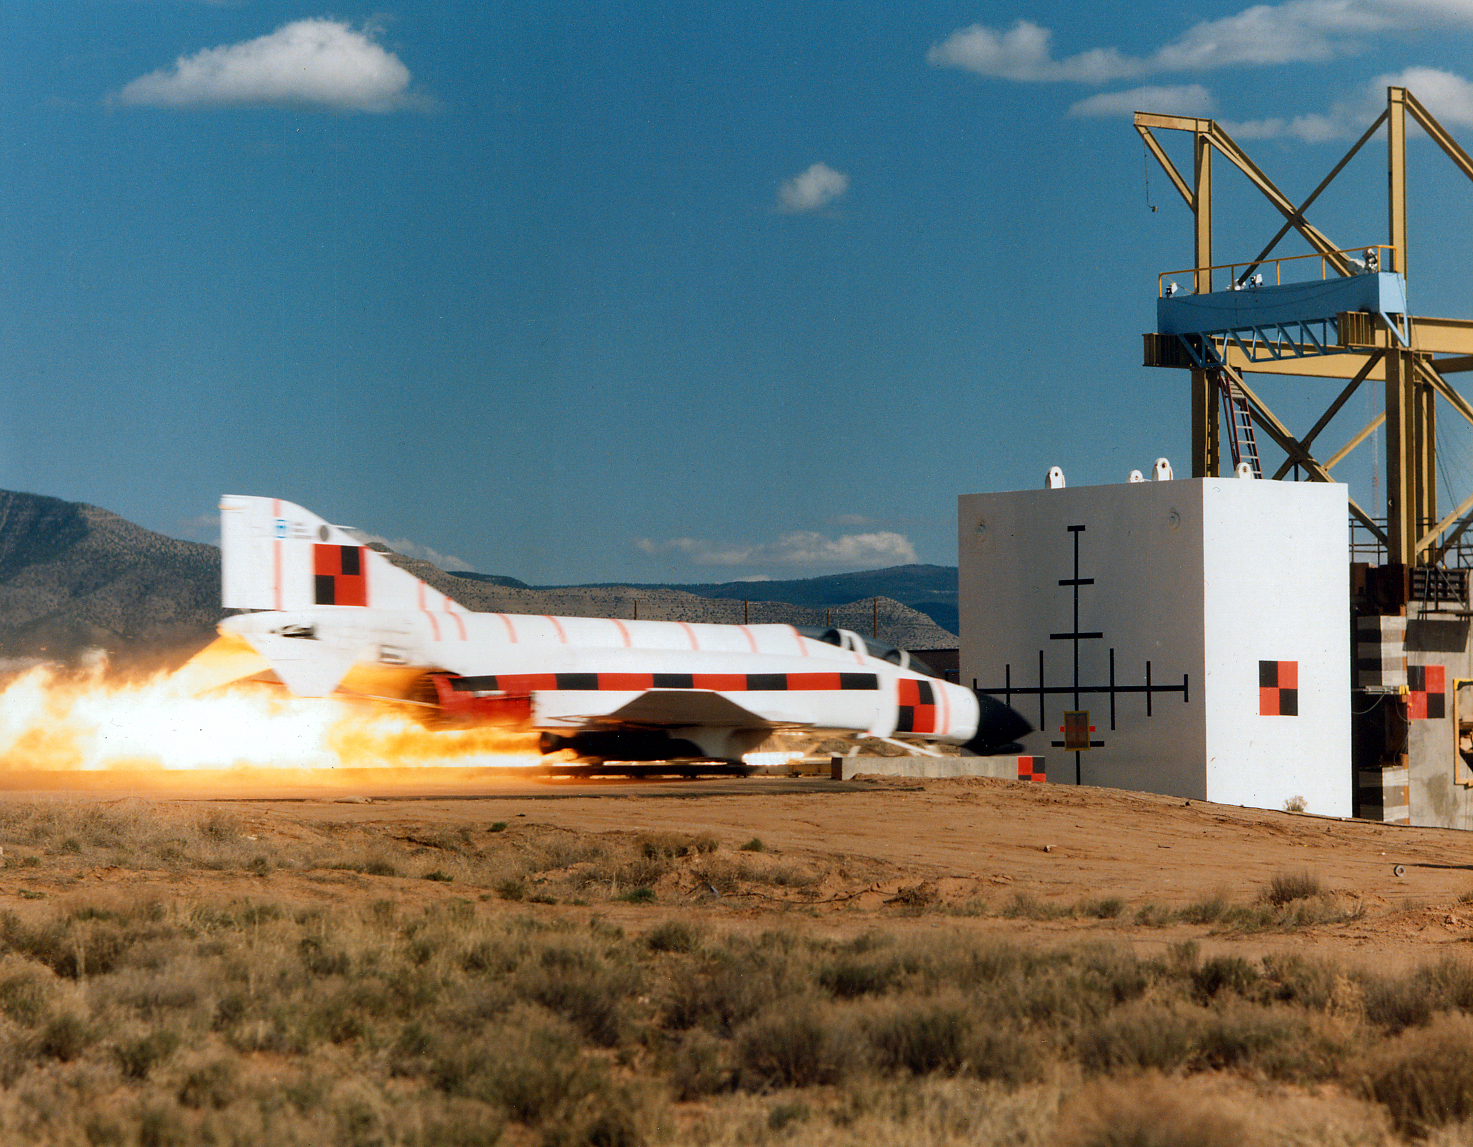
\includegraphics[width=.3\linewidth]{images/Rocket1}
  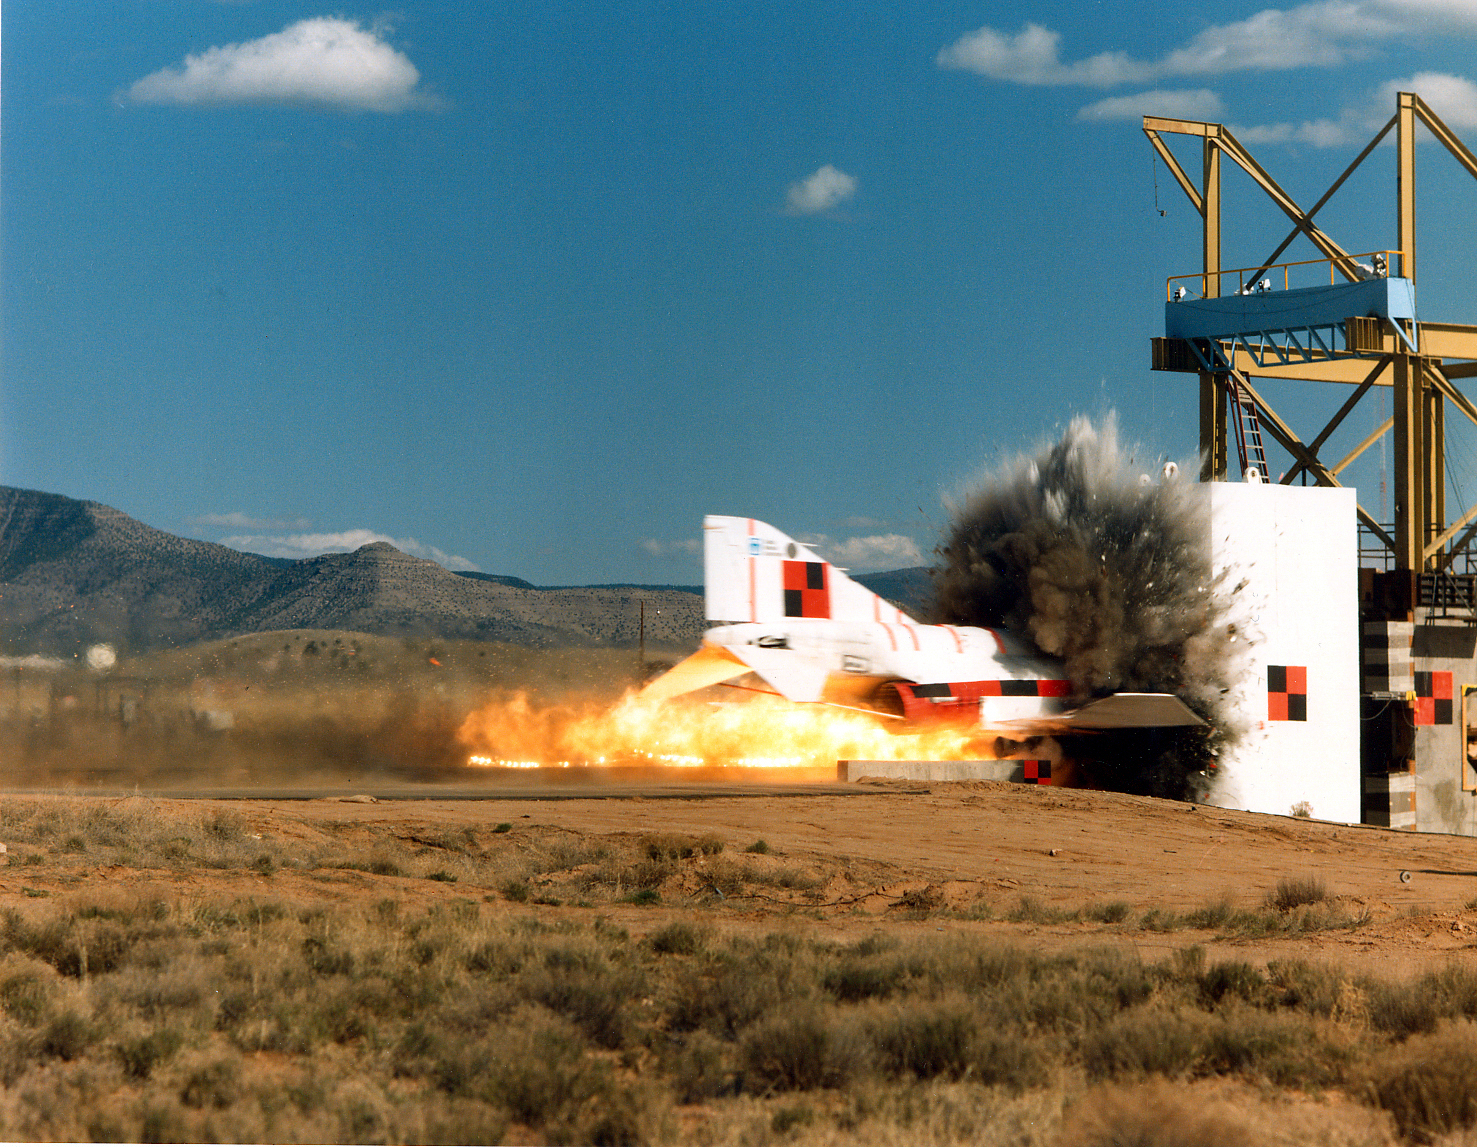
\includegraphics[width=.3\linewidth]{images/Rocket2}
  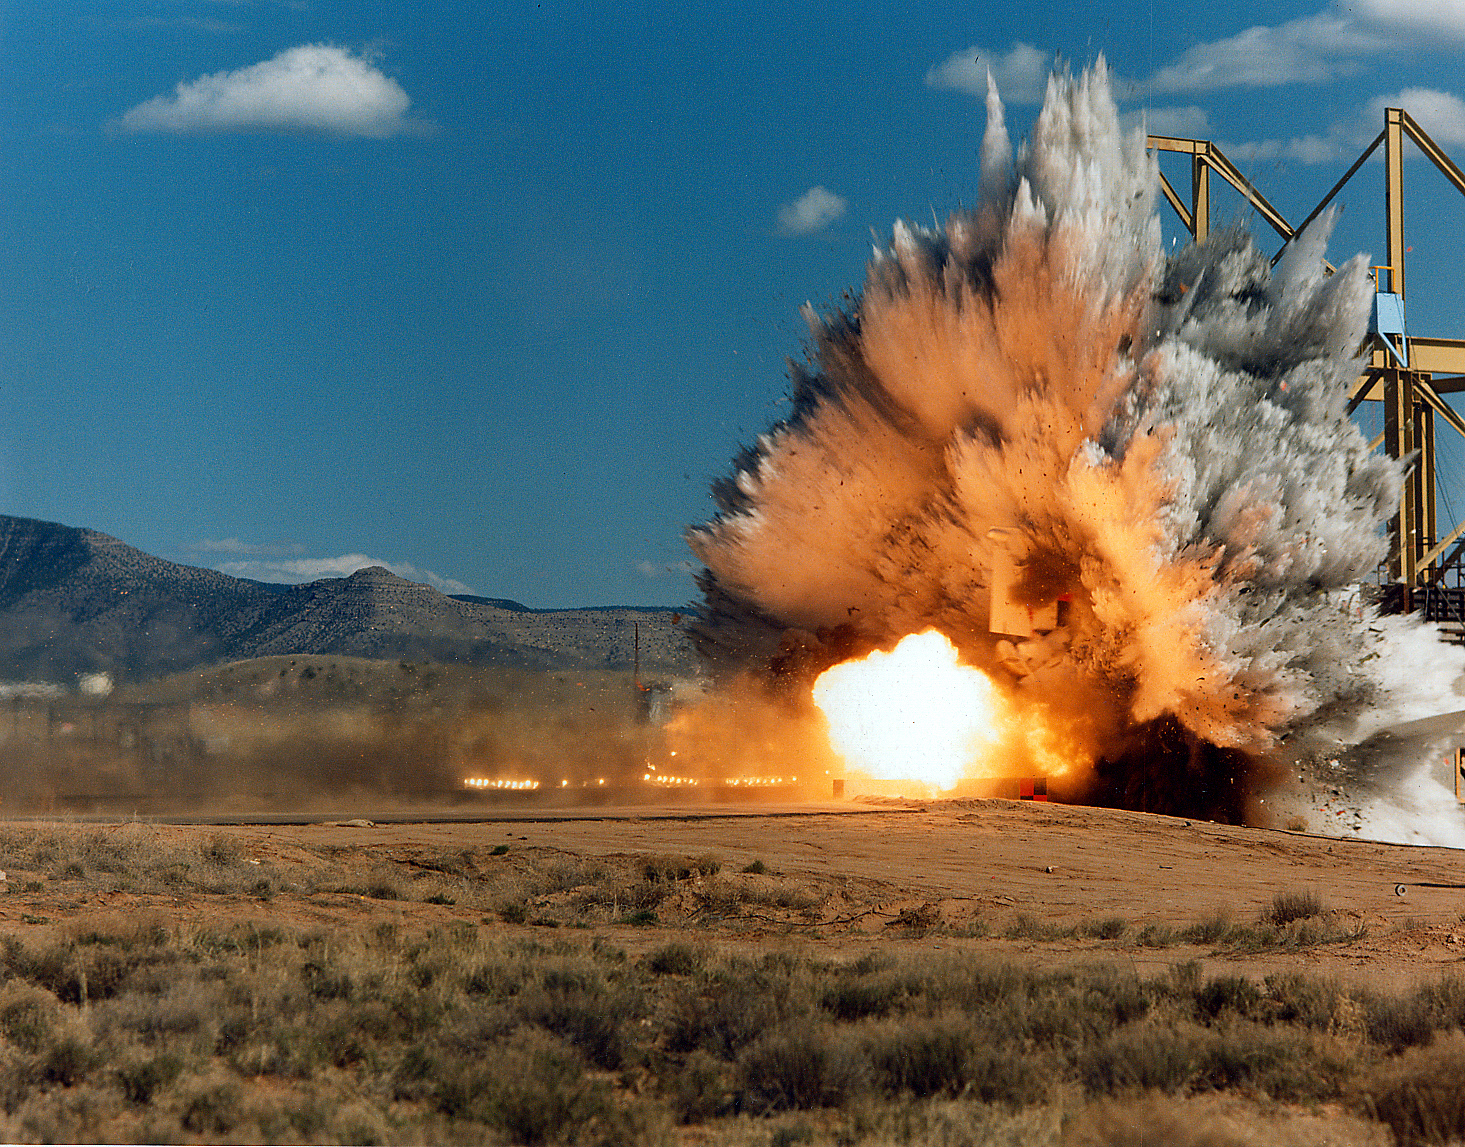
\includegraphics[width=.3\linewidth]{images/Rocket3}
  \caption{This 1988 rocket-sled test has nothing to do with exascale
    computing per se, but it makes for an effective metaphor for the
    ``brick wall'' we anticipate our high-performance computing code to
    collide with.}
  \label{fig:teaser}
}

\begin{document}

\sloppy

\maketitle

%% \twocolumn[\begin{@twocolumnfalse}
%%   %% 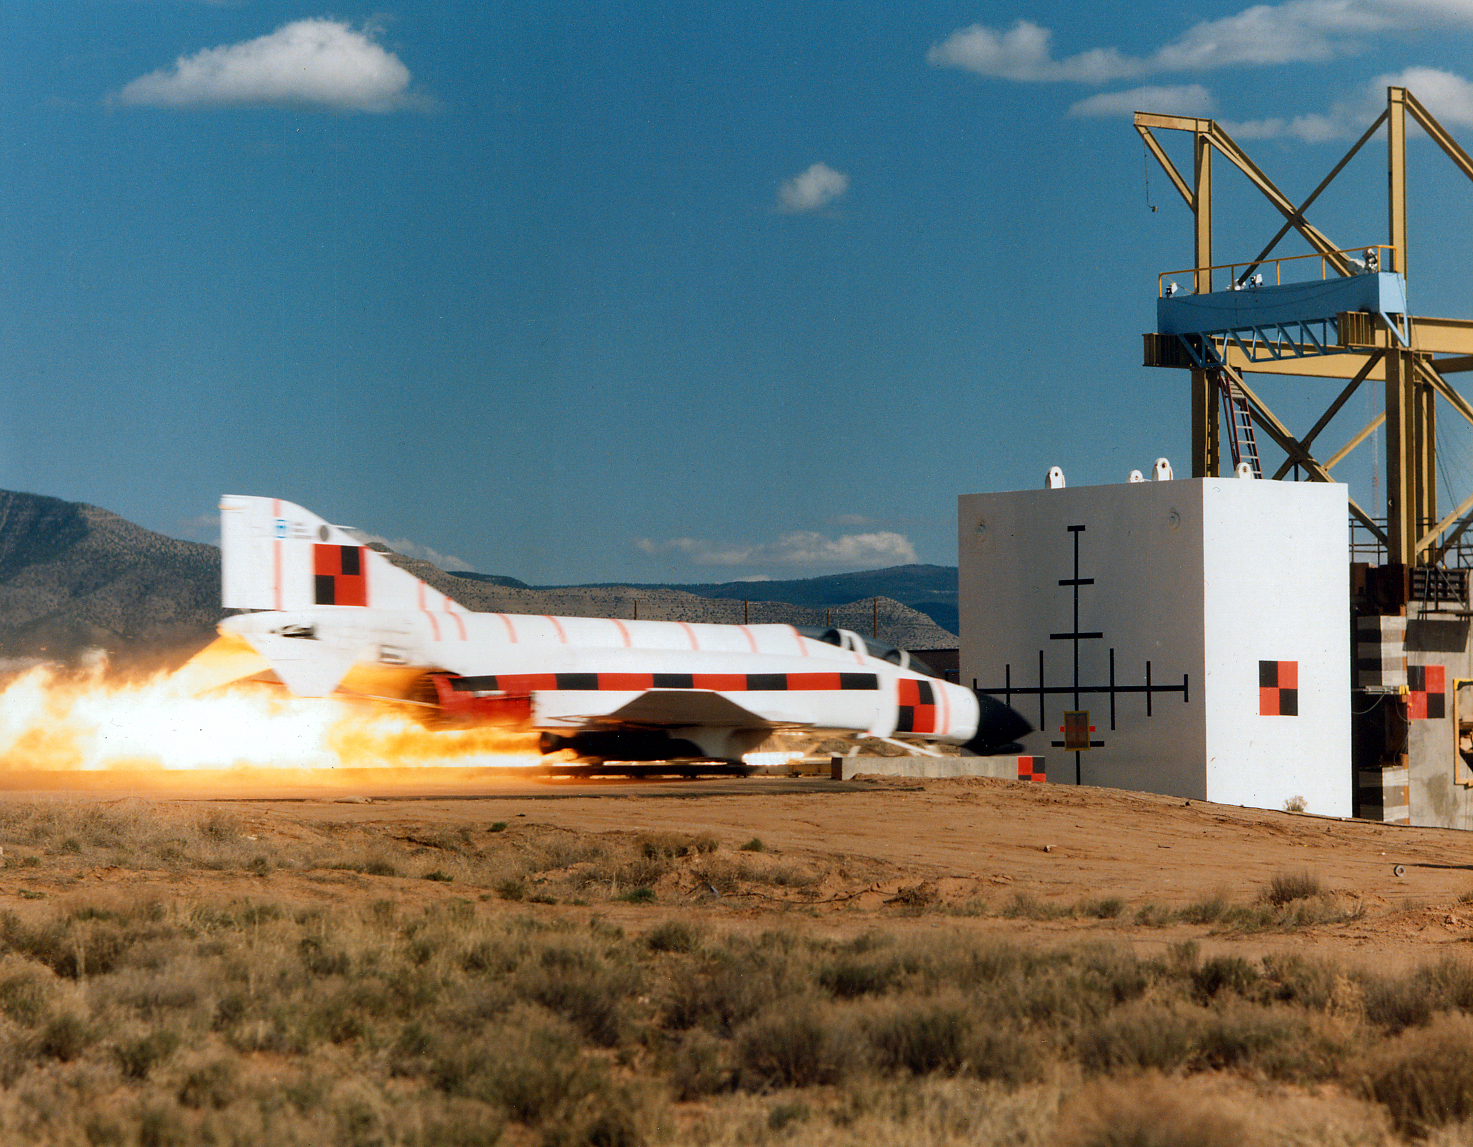
\includegraphics[width=4in]{images/Rocket1}
%%   \centerline{\Large\bfseries This is my manually set ``wide'' title}
%% \end{@twocolumnfalse}]

\begin{abstract}
The predictions for exascale computing are dire.  Although we have
benefited from a consistent supercomputer architecture design, even across
manufacturers, for well over a decade, recent trends indicate that future
high-performance computers will have different hardware structure and
programming models to which software must adapt.  This paper provides an
informal discussion on the ways in which changes in high-performance
computing architecture will profoundly affect the scalability of our
current generation of scientific visualization and analysis codes and how
we must adapt our applications, workflows, and attitudes to continue our
success at exascale computing.
\end{abstract}

\section{Introduction}
\label{sec:Introduction}

This is the introduction.

Figure~\ref{fig:teaser}.

\section*{Acknowledgments}

\noindent
This report is a summary of ongoing work by a great number collaborators
over many institutions.  In particular, I would like to thank the
following: Nathan Fabian and Ron Oldfield from Sandia National
Laboratories; Kwan-Liu Ma, Robert Miller, and Yecong Ye from the University
of California at Davis; Berk Geveci, Utkarsh Ayachit, Robert Maynard, Brad
King, Andrew C. Bauer, Pat Marion, Sebastien Jourdain, David DeMarle, and
David Thompson at Kitware, Inc.; James Ahrens and Jonathan Woodring at Los
Alamos National Laboratory; Scott Klasky and Norbert Podhorszki at Oak
Ridge National Laboratory; Venkatram Vishwanath, Mark Hereld, and Michael
E. Papka at Argonne National Laboratory; Michel Rasquin and Kenneth
E. Jansen at the University of Colorado at Boulder; Ciprian Docan and
Manish Parashar at Rutgers University.


This work was supported in part by the Director, Office of Advanced
Scientific Computing Research, Office of Science, of the U.S. Department of
Energy under Contract No. 12-015215, through the Scientific Discovery
through Advanced Computing (SciDAC) Institute of Scalable Data Management,
Analysis and Visualization.

This work was supported in part by the DOE Office of Science, Advanced
Scientific Computing Research, under award number 10-014707, program
manager Lucy Nowell.

Sandia National Laboratories is a multi-program laboratory operated by
Sandia Corporation, a wholly owned subsidiary of Lockheed Martin
Corporation, for the U.S. Department of Energy's National Nuclear Security
Administration.

\noindent
{\small SAND 2013-XXXX}

%% \bibliographystyle{IEEEtranS}
%% \bibliography{OhShExascale}

\end{document}
